
\documentclass[10pt,aps,prc,twocolumn]{revtex4-1}

\usepackage{tabularx} 
\usepackage{graphicx} 
\usepackage{hyperref}  
\usepackage{amssymb}  
\usepackage{amsmath}  
\usepackage[]{units}

\bibliographystyle{apsrev4-1}

\begin{document}
\title{Balancing Bias and Variance When Selecting Models To Extracting The Proton Radius From Electron Scattering Data} 
%\title{Bias-Variance Trade-Off In Proton Radius Extractions From Electron Scattering Data} 
% a.k.a. How I Learned to Stop Worrying and Love the Bias

\author{Randall Evan McClellan}
\affiliation{Jefferson Lab, Newport News, VA 23606}
\author{Douglas Weadon Higinbotham}
\affiliation{Jefferson Lab, Newport News, VA 23606}
\author{Xuefei Yan}
\affiliation{Duke University, Durham, NC 27708}

\begin{abstract}
Intuitively, phenomenologists often assume that a more complex statistical model will necessarily yield a more 
accurate description of experimental data.   Herein, we analyze this anzats in the context of extracting 
the proton charge radius from simulated charge form factor data.
We will show, that for a given set of data, that a biased parsimonious model can in fact be the better model to use
if it has a significantly smaller variance then the more complex less biased model.
This result provides a simple but important illustration the trade-off between bias and variance that is at the
heart of machine learning.   This concept also forms the basis for regression regularization methods.
We note that those phenomologists using techniques that balance bias and variance,
tend to extract photon radii from electron scattering data that agree with the muonic hydrogen lamb 
shift results, whereas those simply trying to eliminate bias extract larger radii.
\end{abstract}

\maketitle

\section{Introduction}

High precision muonic Lamb shift data have determined the proton radius to 
be √0.84087(39)~fm~\cite{Pohl:2010zza,Antognini:1900ns}.   This result is in stark contrast to the current
CODATA recommended value of 0.875~fm~\cite{Mohr:2015ccw} which comes from an average of atomic 
Lamb shift and electron scattering results.  

While initial efforts to understand this puzzle focused on the details muonic result, attention has
now turned to re-examining the atomic and electron scattering results.   In fact, the first of the
new generation of published atomic result is in fact in statistical agreement with the muonic 
result~\cite{Beyer79} though preliminary results from another group agrees with the classic atomic 
results~\cite{fleurbaey:tel-01633631}.

For electron scattering, the puzzle has also become unclear with extractions of the proton 
radius ranging from relatively parsimonious fits of 
low Q$^2$ data~\cite{Griffioen:2015hta,Horbatsch:2016ilr,Higinbotham:2015rja} to 
extremely complex models with more than fifty free parameters~\cite{Bernauer:2013tpr,Lee:2015jqa}.   
As nicely illustrated in the work of Krauth~{\it{et al.}}~\cite{Krauth:2017ijq}, the 
new parsimonious fits tend to agree with the muonic results while the more complex fits 
are generally in agreement with the CODATA value.

For the electron scattering data, the proton's charge radius, $r_p$, is extracted
by determining the slope of the electric form factor as the four-moment transfer, $Q^2$,
approaches zero.   The relation between this slope and 
the radius is defined to be
$$
G_E(Q^2)
   =  1
   +  \sum_{n\ge 1} \frac{(-1)^n}{(2n+1)!}
      \left\langle r^{2n} \right\rangle \, Q^{2n} \>.
$$
Hence, $r_p$ can be determined from
$$
  r_p \equiv \sqrt{ \langle r^2 \rangle}
   = \left( -6  \left. \frac{\mathrm{d} G_E(Q^2)}{\mathrm{d}Q^2}
    \right|_{Q^{2}=0} \right)^{1/2} \>.
 $$
Of course, electron scattering cannot reach the exact $Q^2 = 0$ limit; thus,
an extrapolation is required to extract the charge radius from the experimental data.

One of the criticisms of the parsimonious extractions of the proton radius is the prescience of bias~\cite{Sick:2017aor}.
with an implication that bias needs to be avoided in order to successfully extract the true radius from the data.
In fact, the rejection of statistical models based solely on bias was explicitly stated in the 
classic Monte Carlo study of Borkowski~{\it{et al.}}~\cite{Borkowski:1975}. 
We will show in this work that when using a Monte Carlo study to test a statistical model's ability
to extract the proton radius, one needs to in fact consider both bias and variance.

\section{Bias}

A very straight forward example of bias being used to rule out simpler models can be found in a Z. Physik
article from 1975~\cite{Borkowski:1975}; and while an older research article, its very strong conclusions are still 
noted to this day~\cite{Sick:2017aor} and a similar exercises have been done with other functions 
in Kruas~\textit{et al.}~\cite{Kraus:2014qua}.
As noted in~\cite{Hogg:2010yz}, the use of even an approximate generative model can be extremely 
important in understanding thus it is worth while to revisit this problem using the standard dipole 
function used by Borkowski~{\it{et al.}}. 

The example problem, as presented in the Z. Physik paper, is simple to reproduce.   
Randomly generate sets of faux change form factor faux in steps of $\unit[0.05]{fm^{-2}}$ from $\unit[0.1]{fm^{-2}}$ to 0.4, 0.8, 1.2,
and $\unit[1.6]{fm^{-2}}$ using the standard dipole function:
\begin{equation}
\label{sd}
\mathrm{G_D}(Q^2) = ( 1 + Q^2/(\unit[18.27]{fm^{-2}}))^{-2}.
\end{equation}
Perform fits on the resulting sets of faux data with linear and quadratic functions. The entire procedure is
then repeated many times to determine the mean of the extracted radii for each model. Table~\ref{ztable} reproduces the table found in the
Z. Physik article using python on a modern computer yielding only minor differences.
As the table clearly shows, the mean of $10^6$ linear fits is biased. 
Therefore, the authors conclude that the linear models should be rejected in favor of the lower-bias quadratic function.
They then proceed to extract the proton charge radius from real data using a five parameter fit: a quadratic charge form factor and three floating normalizations.

\begin{table}
\label{ztable}
\caption{The following table shows the mean a$_0$ and radius terms from doing $10^6$ Monte Carlo simulations
for each range
where Eq.~\ref{sd} was used to generate faux data in $\unit[0.05]{fm^{-2}}$ steps with each points randomized using
0.5\% normal distribution.   The results clearly indicate that the linear fits are biased.   The input
radius was \unit[0.8113]{fm} (an a1/a0 term of $\unit[0.1097]{fm^{-1}}$) and an a0 of one.}
\begin{tabular}{c|cc|cc} \hline
interval       & \multicolumn{2}{c|}{linear fit} & \multicolumn{2}{c}{quadratic fit}  \\
fm$^{-2}$      & a$_0$      & radius          & a$_0$    & radius \\ \hline
 0.1 -- 0.4 & 1.000& 0.79& 1.000& 0.81 \\
 0.1 -- 0.8 & 0.999& 0.78& 1.000& 0.81 \\
 0.1 -- 1.2 & 0.997& 0.77& 1.000& 0.81 \\
 0.1 -- 1.6 & 0.996& 0.76& 1.000& 0.81 \\ \hline
\end{tabular}
\end{table}

\section{Variance}

While the mean of the results is indeed correct; when we run an experiment we typically do no get to run it $10^6$ times.
In particular in nuclear physics, the experiments are few and far between thus we need to carefully consider variance as
well as the bias when picking the statistical model to use.
%
%If the authors of the Z. Phys. paper had decided to focus on variance instead of bias, they would have come to a very
%different conclusion.
%
%\begin{table}
%\label{ztable}
%\caption{The following table shows the variance of the a$_0$ and radius terms from doing $10^6$ Monte Carlo simulations
%for each range
%where Eq.~\ref{sd} was used to generate faux data in $\unit[0.05]{fm^{-2}}$ steps with each points randomized using
%0.5\% normal distribution.   The results clearly indicate that the quadratic fits have a large variance.   The input
%radius was \unit[0.8113]{fm} (an a1/a0 term of $\unit[0.1097]{fm^{-1}}$) and an a0 of one.}
%\begin{tabular}{c|c|c} \hline
%interval       & \multicolumn{1}{c|}{linear fit} & \multicolumn{1}{c}{quadratic fit}  \\
%fm$^{-2}$   & sigma [fm]         &  sigma [fm] \\ \hline
% 0.1 -- 0.4 & 0.0184&  0.1094 \\
% 0.1 -- 0.8 & 0.0095&  0.0281 \\
% 0.1 -- 1.2 & 0.0110&  0.0138 \\
% 0.1 -- 1.6 & 0.0136&  0.0085 \\ \hline
%\end{tabular}
%\end{table}
%
%
Table~\ref{fulltable} shows more complete picture of the simulation results where the variance is shown along with the bias.
This table in fact shows nearly a textbook illustration of the trade-off between variance and bias with the simple fits
having a relatively high bias with a low variance while the quadratic fits have a low bias and high variance.

\begin{table*}
\label{fulltable}
\caption{The input radius was 0.8113 fm (an a1/a0 of $\unit[0.1097]{fm^{-1}}$).}
\begin{tabular}{cc|cccccc|cccccc} \hline
Data   & Range     & \multicolumn{6}{c|}{linear fit}                       & \multicolumn{6}{c}{quadratic fit}                    \\ 
Points & fm$^{-2}$ &   a0  & Radius&  a1/a0 &  Bias  & Sigma &  RMSE  &   a0  & Radius& a1/a0  &  Bias  & Sigma &  RMSE \\  \hline
7      & 0.1 -- 0.4 & 0.9995& 0.7948& -0.1053& -0.0044& 0.0184& 0.0189 & 1.0000& 0.8063& -0.1084& -0.0013& 0.1094& 0.1094\\
15     & 0.1 -- 0.8 & 0.9987& 0.7828& -0.1021& -0.0076& 0.0057& 0.0095 & 1.0000& 0.8096& -0.1092& -0.0005& 0.0281& 0.0281\\
22     & 0.1 -- 1.2 & 0.9975& 0.7712& -0.0991& -0.0106& 0.0030& 0.0110 & 0.9999& 0.8089& -0.1090& -0.0007& 0.0138& 0.0138\\
31     & 0.1 -- 1.6 & 0.9959& 0.7600& -0.0963& -0.0134& 0.0019& 0.0136 & 0.9998& 0.8075& -0.1087& -0.0010& 0.0085& 0.0085\\ \hline
\end{tabular}
\end{table*}

\begin{figure}[htbp]
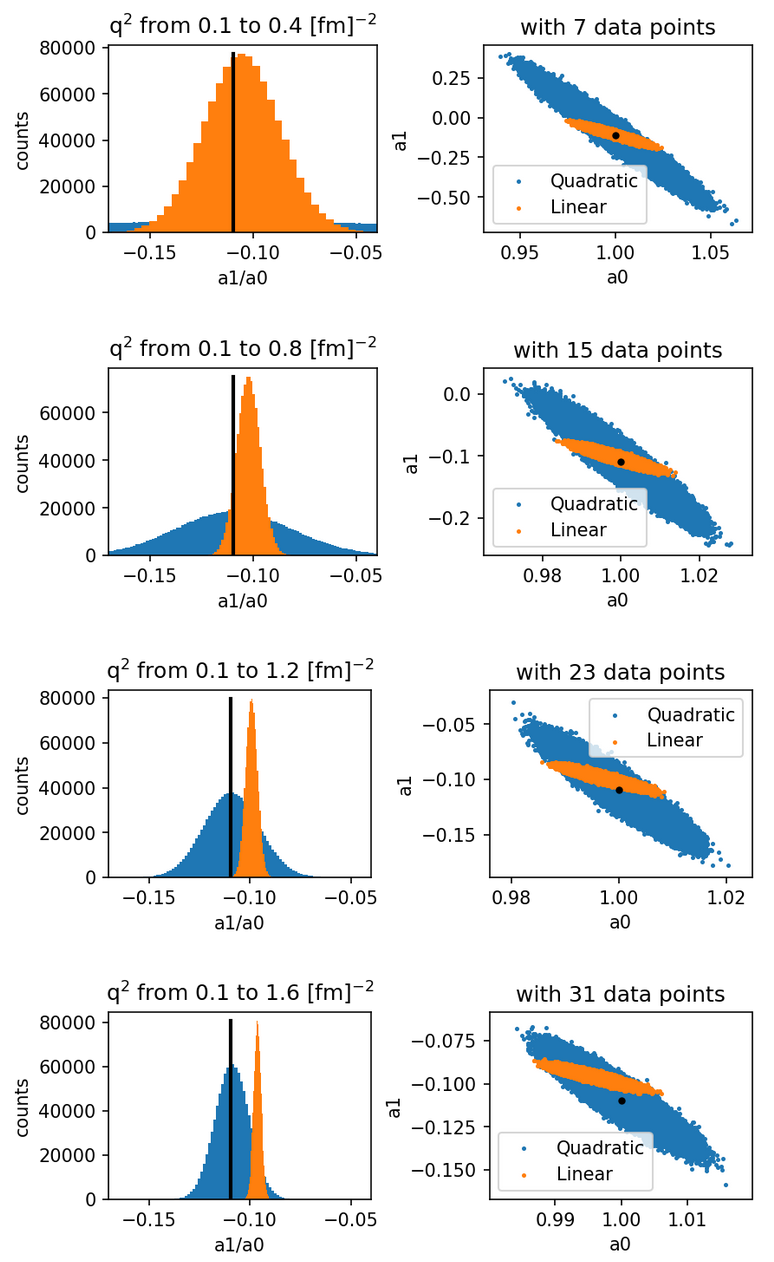
\includegraphics[width=\columnwidth]{Figure/zresult.png}
\caption{A graphic representation of the Monte Carlo results showing how the linear fits tend to have a reliatvely
high bias though a low variance while the quadratic fits tend to a a reliatively low bias but a large variance.}
\end{figure}

\begin{table*}
\label{equaldatatable}
\caption{Same as before, but now with equal number of data points of each range.}
\begin{tabular}{cc|cccccc|cccccc} \hline
Data   & Range     & \multicolumn{6}{c|}{linear fit}                       & \multicolumn{6}{c}{quadratic fit}                    \\ 
Points & fm$^{-2}$ &   a0  & Radius&  a1/a0 &  Bias  & Sigma &  RMSE  &   a0  & Radius& a1/a0  &  Bias  & Sigma &  RMSE \\  \hline
31& 0.1 - 0.4 & 0.9995& 0.7951& -0.1054& -0.0043& 0.0098& 0.0107 & 1.0000& 0.8090& -0.1091& -0.0006& 0.0629& 0.0629 \\
31& 0.1 - 0.8 & 0.9987& 0.7829& -0.1021& -0.0076& 0.0041& 0.0086 & 1.0000& 0.8099& -0.1093& -0.0004& 0.0208& 0.0208  \\
31& 0.1 - 1.2 & 0.9974& 0.7712& -0.0991& -0.0106& 0.0026& 0.0109 & 0.9999& 0.8089& -0.1091& -0.0006& 0.0121& 0.0121  \\
31& 0.1 - 1.6 & 0.9959& 0.7600& -0.0963& -0.0134& 0.0019& 0.0136 & 0.9998& 0.8076& -0.1087& -0.0010& 0.0085& 0.0085  \\  \hline
\end{tabular}
\end{table*}

\section{Goldilocks Dilemma}

For any given statistical model, the goal is to find the optimal balance between bias and variance.   
In general, this can be written as:
\begin{equation}
\frac{d Bias^2 }{ d Complexity} = \frac{- d Variance }{ d Complexity }
\end{equation}

Thus going back to Table~\ref{fulltable} and checking the root mean square error, one can see that for the four ranges
one finds the 0.1 -- 0.8 range is actually optimal for the linear model and the 0.1 -- 1.6 range is optimal for the quadratic model. 
This is in complete contrast to the conclusion one draws when only considers bias as presented in Table~\ref{ztable}
though constant with the observation that the optimal specific form of the parameterization may depend on the $Q^2$ region
being fit~\cite{Alberico:2008sz}.
\begin{figure}
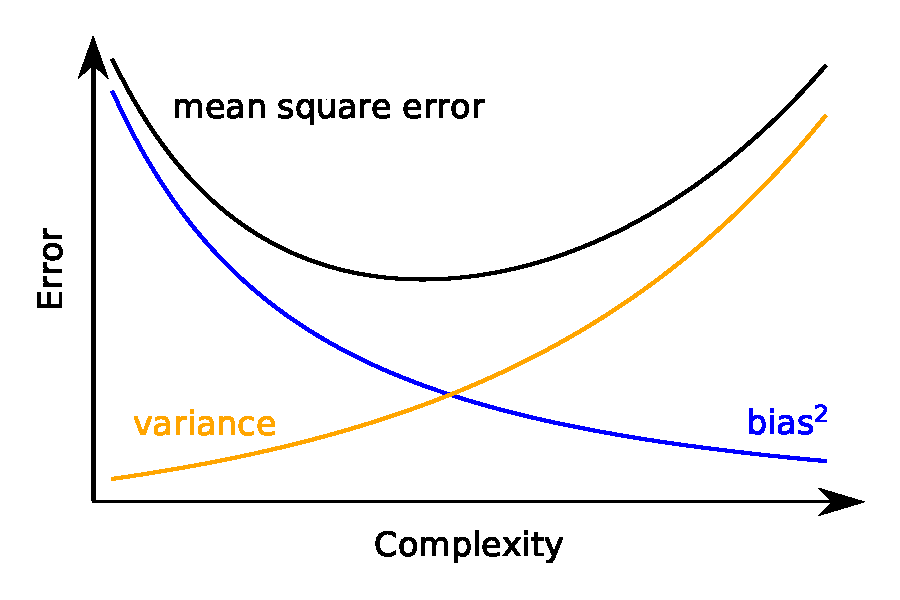
\includegraphics[width=\columnwidth]{Figure/biasvariance-clean.pdf}
\caption{An illustration of the trade-off between bias and variance when selecting a statistical model.   Simple models
will have low variance but high bias (under-fitting) while complex models will have low bias but high variance (over-fitting).   
It is this trade-off that one seeks to balance.   While with repeated  Monte Carlo simulations it is trivial to find the optimal
predictive model for a give set of data; in the real world true model is typically unknown and one only gets preform a very limited number
of experiments and thus one relys on using real data and statistical methods for model selection~\cite{Hastie:2009}.
}
\end{figure}

It is interesting to repeat the Monte Carlo simulation for equal number of data points within each range
especially since, for any given experiment, the elastic scattering cross sections are significantly higher as lower values
of Q$^2$.

As shown in Table~\ref{equaldatatable}, the picture is even grayer as the root mean square error of the linear 
fit is nearly equal to the quadratic thus, assuming standard dipole was the true generating function,  experiments
with 31 data point and an uncertainty of 0.005 per point over a range of 0.1 to 0.8 and a different experiment
over a range of 0.1 to 1.6 would produce nearly identical if all other things were equal.

In this case, the choice of the parsimonious modeler to use the low Q$^2$ data would like be driven by the recognition that as Q$^2$ increases
the extraction of a charge form factor is complicated by the growing influence of the magnetic form factor while the use of the larger Q$^2$
range would likely be driven by a desire to form a more complete picture of the proton's structure 
(e.g. one may be interested in not only in the proton's radius but also higher order moments).

%\begin{equation}
%\sigma / \sigma_{Mott} = eps G_E^2 + tau G_M^2
%\end{equation}

\begin{figure}
\label{zoptimized}
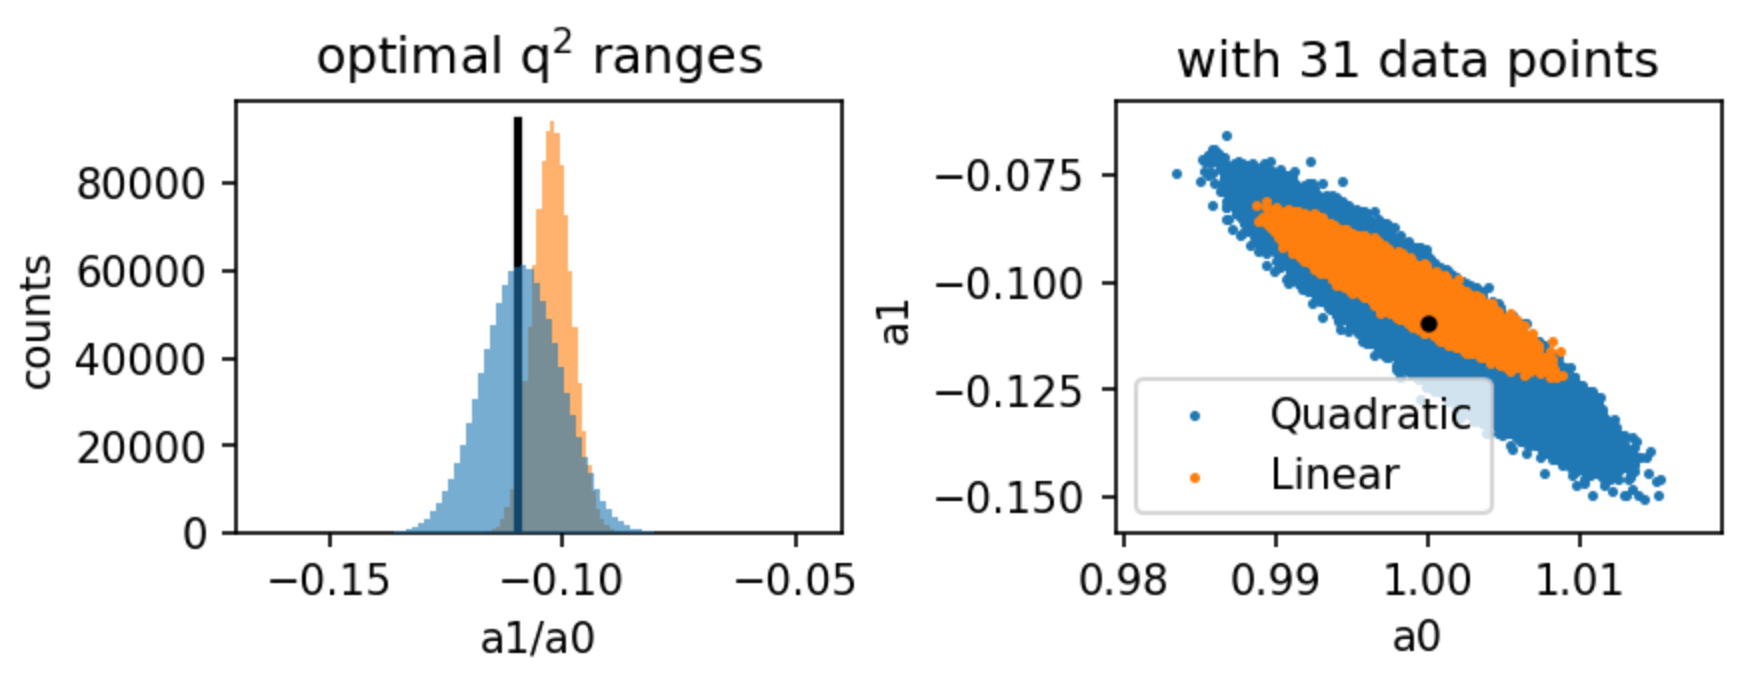
\includegraphics[width=\columnwidth]{Figure/zoptimized.png}
\caption{Shown is the result of million simulations and fits of linear fits  0.1 -- 0.8~fm$^{-2}$ 
and quadratic fits 0.1 -- 1.6~fm$^{-2}$ both with 31 equally spaced data points.    Using root mean
square error as the matrix, neither example is significantly better then the other for exacting the proton
radius   This is analogous to a dart game between two equally skilled players though one who hits the bulls eye more 
often yet has a large spread (low bias but high variance) and another equally skilled player who has a tighter cluster of hits
but an offset (high bias but low variance).}
\end{figure}

The above illustration in fact suggests there are indeed two path forward for the modeler.   Either use simple models and extremely low Q2 
data or use more complex models that cover larger ranges of data.   It is worth noting that in order to use larger ranges
of experimental data, one will need to model not only the charge form factor but also the exact details of  magnetic form factor
will start become quite important.


\section{Model Selection and the Modern Debate}

While this classic Monte Carlo example problem is over 40 years old, it actually points to exactly the split in 
the current electron scattering proton radius extraction procedures.     The parsimonious modelers, who are 
focused solely on extracting a radius, have focused in on the low Q$^2$ region accepting accepting a slightly higher 
level of bias in exchange for low variance while those modelers who are interesting in extracting more information 
about the proton (i.e. higher order moments) fit longer Q$^2$ ranges and have
focused on complex models which while lower in bias come at a cost of higher variance.  
It fact, the result of increasing Q$^2$ ranges requiring increasing complexity have resulted in
an uncertainty in the extracted radius 
stuck at $\approx \unit[0.01]{fm}$ since L.~Hand~\textit{et al.}'s original fit in 1963~\cite{Hand:1963zz}.

Also, since we don't know the true model, one cannot in general calculate the RMSE; so while Monte Carlo exercises 
like the one described herein are extremely useful for making sets are models; in the end, the data must be used 
to select the approximate model. 
For this one can relay on statistical modeling techniques such as chi2, reduced chi2, F-tests, A.I.C., B.I.C. 
to guide our selection of regression models and/or use theoretical constraints.

In fact, statistics books warn about drawing too strong an inference from these types of Monte Carlos.   For example,
just because the linear model has a negative bias when compared to standard dipole, does not imply that it has a negative bias
to all possible models.
In fact, the Z.Physik paper itself rules out the very model it was using for model building: i.e. 
drawing very strong conclusions from the standard dipole function with its \unit[0.81]{fm} radius 
yet their five parameter fit (two charge form factor parameters and three normalization parameters)
gave a radius of \unit[0.87]{fm}.

Looking back to our example function, one can see that the range of the 
Saskatoon data (0.1 -- 0.8 fm$^{-2}$) could in fact be a reasonable
choice for extracting a radius and as shown much later if one redoes 
the Z.Physik fits but adopts the Saskatoon linear procedure one finds
a radius of \unit[0.84]{fm}~\cite{Higinbotham:2015rja}.   

\section{Beyond Polynomial Expansions}

While one can continue to increase the $Q^2$ range of the data, one will find that 
higher and higher order polynomials are required
to describe the data and as shown in~\cite{Kraus:2014qua}, but this leads to ever increasing variance 
and instability as real data isn't perfectly normally distributed as in these example Monte Carlo distributions.

To try to avoid these issues, one can implement a bounded least squares fit based on a 
physics argument~\cite{Horbatsch:2016ilr} 
or try a purely statistical approaches such as machine learning regression such as stepwise regression~\cite{Higinbotham:rja},
though it would be far more satisfying to simply find a function that has both low bias and low variance over a large 
range of $Q^2$.  In particular, rational functions~\cite{Kelly:2004hm,Puckett:2017flj} and continued 
fractions~\cite{Sick:2003gm} are known to extrapolate well and should be further investigated.

\section{Summary}

The concept of a bias-variance trade-off is key to regularization techniques such as stepwise regression, 
ridge regression and statistical lasso.    By accepting some bias, these techniques tend to achieve a far 
superior mean square error then the unregulated ordinary least squares solution of the same complexity.     

For the specific example of electron scattering, we have revisited a classic Monte Carlo study and shown
the practice of simply concluding that the model with a higher predictive validity 
is truer is not a valid assumption; and in fact, the  parsimonious model can in fact 
have the higher predictive validity depending on the exact range and precision of the data.
Further details about the difference between descriptive and predictive modeling can be 
found in Shmueli's article ``To Explain or to predict''~\cite{Shmueli:2010}.

This work was supported by the U.S.  Department of Energy contract DE-AC05-06OR23177
under which Jefferson Science Associates operates the Thomas Jefferson National 
Accelerator Facility.    {\bf{Add Duke contract.}}

\bibliography{elastic}

\end{document}
